\section{Evaluation} \label{sec:Evaluation}
This chapter includes the detailed evaluation of the final application to get a conclusion about the applicability of the approach in reality and the trustworthiness of the light direction estimation. Thus, all test image of the second batch and some of the first batch were used three times to estimate a light vector with the application. Then all resulting vectors are printed into the images and compared. Every surface normal $\vec{N}$ of a path is printed in red along the green sub-contour while the patch light vectors $\vec{L}^n$ are visualised by white lines. The final estimated light vector $\vec{v}$ is displayed as a blue line. 

As mentioned in Section \ref{sec:approaches}, two \textcolor{red}{=THREE, vielleicht müssen wir da nochmal schreiben, dass der erste approach nicht ausgewertet wird, weil er zu sehr ungenauen ergebnissen führt, weil die Refletkion als konstant angenommen wird} approaches were implemented and have to be evaluated as a consequence. However, it turned out that the results of both \textcolor{red}{evaluated} approaches seem to be almost similar and therefore this evaluation focus on the first approach which appear to be more suitable. The same similarity could be observed between the results of the first and second batch of test images. Hence, the second batch is preferred because it is simpler and thus a better reproducibility. All visual observations of the evaluation are listed, discussed and rated in the following sections.

\subsection{Evaluation 2. Approach}
During the generation of resulting $\vec{v}$ from the test images, it became obvious that almost correctly light vectors could be calculated with the approach. As shown in Figure~\ref{fig:goodRes}, the final light vector $\vec{v}$ almost points into the direction of the sun clock shadow. Little variations can be related to image noise and numeric rounding. Some results show vectors that are flipped exactly horizontally into the opposite direction.
\begin{figure}[H] 
	\center 
	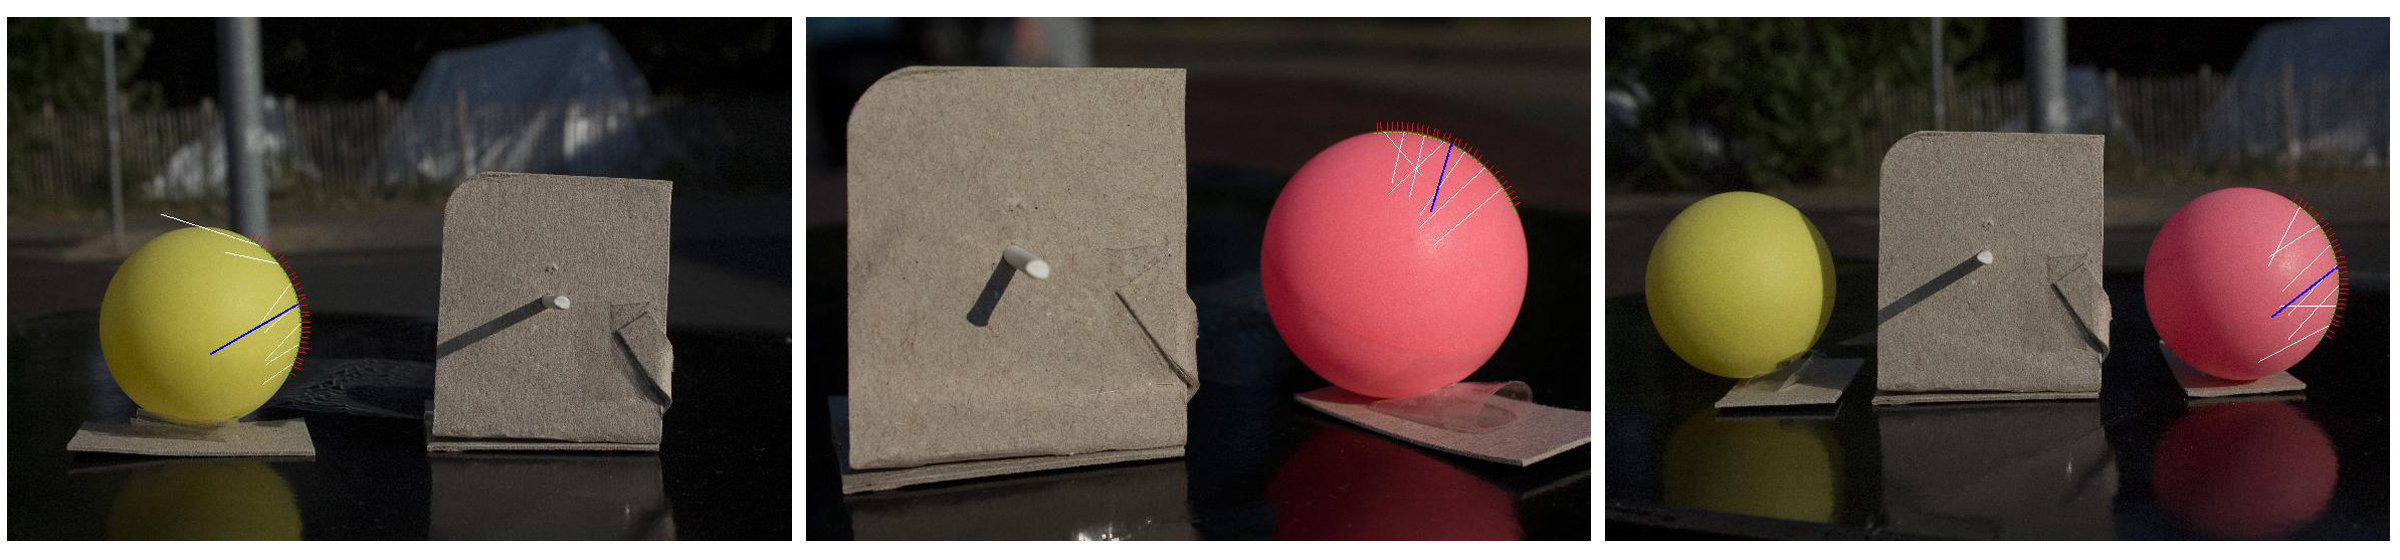
\includegraphics[width=\linewidth]{Images/Korrekte_Lightvectoren.jpg}	
	\caption[Bildunterschrift]{Correct estimated light vectors.}	
		\label{fig:goodRes}	
\end{figure}
However, most of the approximated light vectors $\vec{v}$ despite the few mentioned correct ones, are significantly wrong. Figures~\ref{fig:difDistance} and \ref{fig:divLightDirect} show that the estimated patch light vectors $\vec{L}^n$ are not coherent and thus the final $\vec{v}$ has huge differences to the validated light direction of the sun clock as well. It is obvious that the norm of $\vec{v}$ does not correlate to the length of the sun clock shadow. All these mentioned estimation errors appear to be randomly and without any correlations that can be determined. 

To consider those correlations, the second batch of test images is split into two groups. The first part contains images that are captured with increasing distances to the object of interest (see Figure~\ref{fig:difDistance}). In comparison to the general observations, the quality of these results turned out to be almost similar and the lack of coherence is still given. Thus, it can be assumed that the size of image section and the related number of patches have no big influence to the estimation error and proofs a low robustness of the approach. 
\begin{figure}[H] 

	\center 
	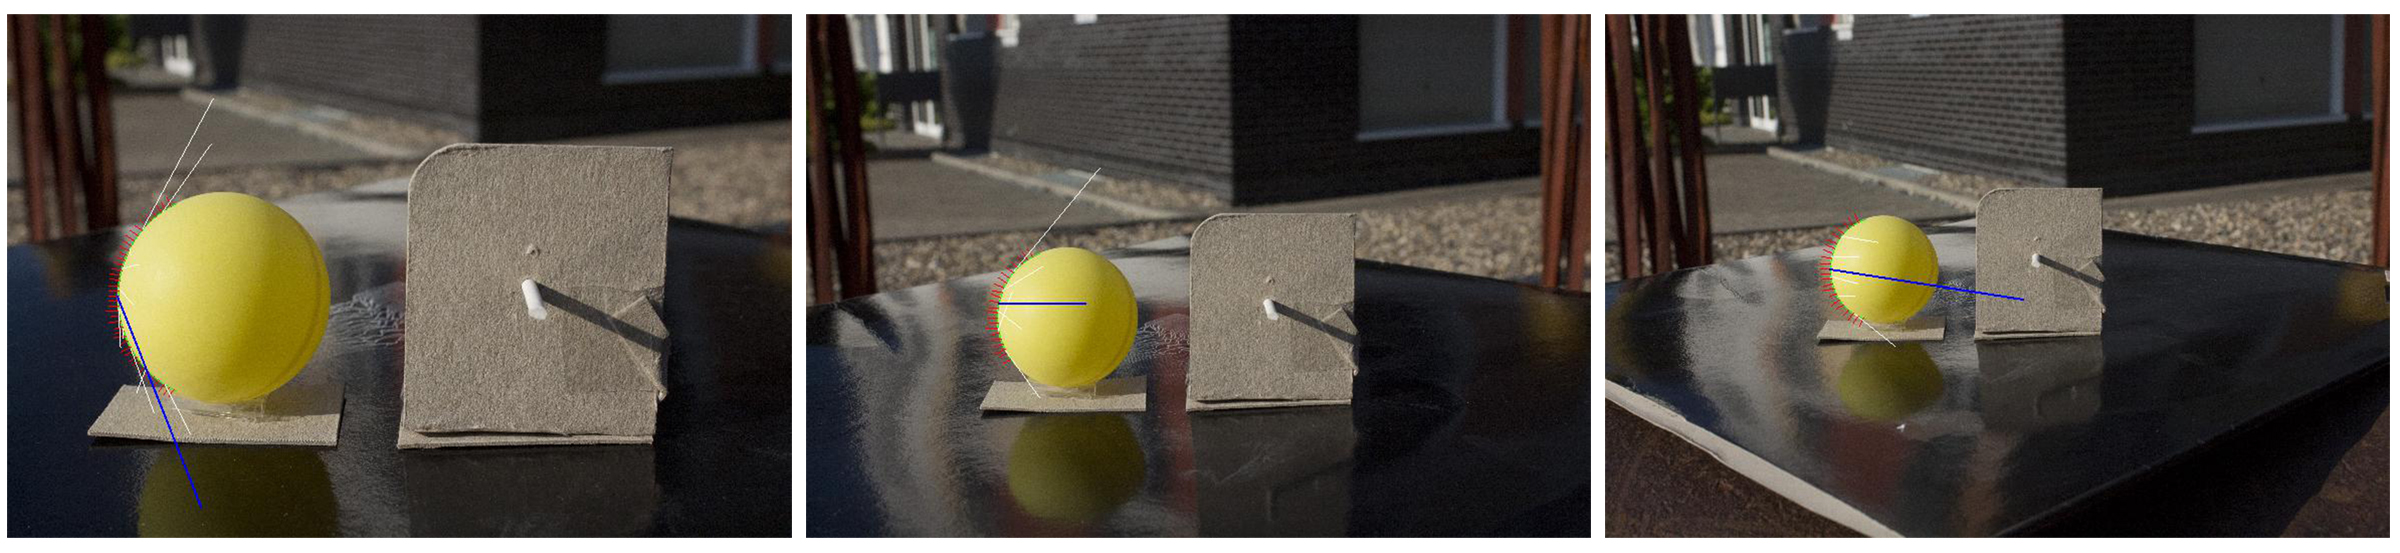
\includegraphics[width=\linewidth]{Images/versch_Anstaende.jpg}
	\caption[Bildunterschrift]{Results of images with increasing distances.}
		\label{fig:difDistance}		
\end{figure}
The second part includes images with various light direction to consider if the Johnson approach has problems with special circumstances like the angle between $\vec{N}$ and $\vec{L}$ or a certain light directions. In Figure~\ref{fig:divLightDirect} is a collection of some examples of this group shown. It gives the assumption that the algorithm is correctly implemented because the coherence is in the same range than with the general results. No significantly differences can be figured out related to certain light directions or angles and thus it can be assumed that the least square problem is correctly implemented and the high error rate is related to external influences like image noise, surface reflections and a huge ambient light proportion. \textcolor{red}{ergibt sich die hohe error rate nicht eher weil die Annahmen schrott sind? Oder verstehe ich da was falsch?}
\begin{figure}[H] 

	\center 
	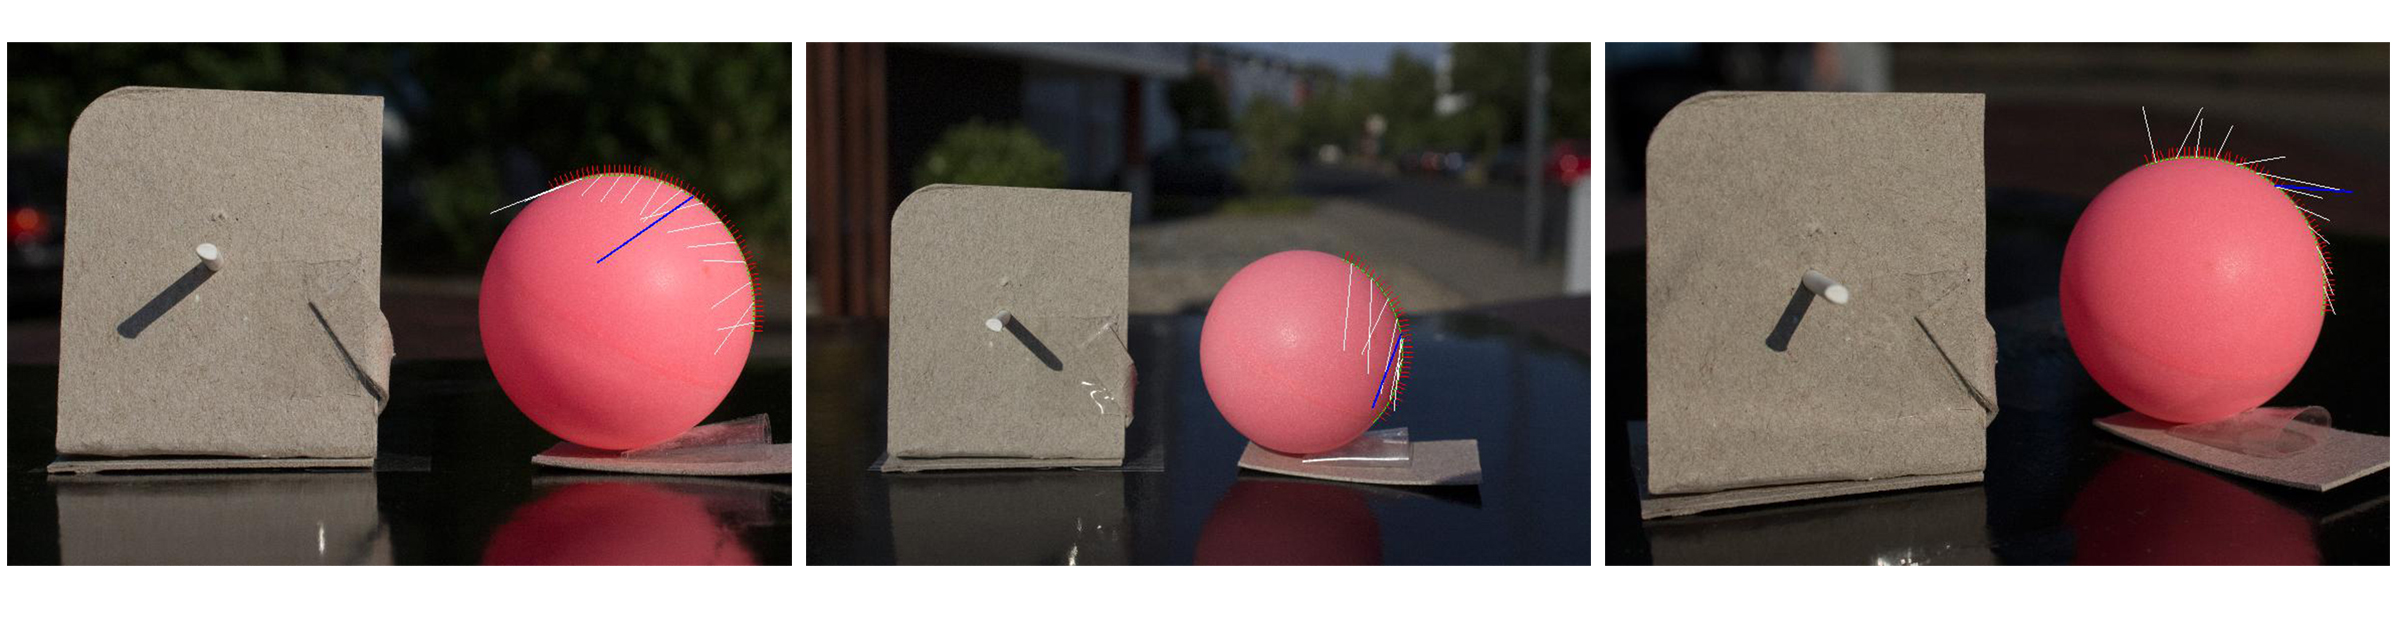
\includegraphics[width=\linewidth]{Images/versch_Lichtrichtungen.jpg}
	\caption[Bildunterschrift]{Results of images with various light directions.}
		\label{fig:divLightDirect}		
\end{figure}

This assumption is affirmed by the observation of the sub-contour position influence. The best results can be generated if the sub-contour fits closely and symmetrically around patch with highest intensity as shown in Figure~\ref{fig:goodRes}. All successful estimations are generated from sub-contours whose selections have the patch of maximum mean intensity almost in the middle and includes a selection of patches that are related to the light direction of the infinitive light source without any shadow parts. The length of these sub-contours needs to be longer if the light incidence is less planar. 

Nonetheless, the success is quite sensible as shown in Figure~\ref{fig:subcontourRes}. Slightly variances in the length and position of the sub-contour results in significant changes of the light vector and its length. This proofs also that correct results seems to be occasional and can not much forced by user intervention. 

\begin{figure}[H] 

	\center 
	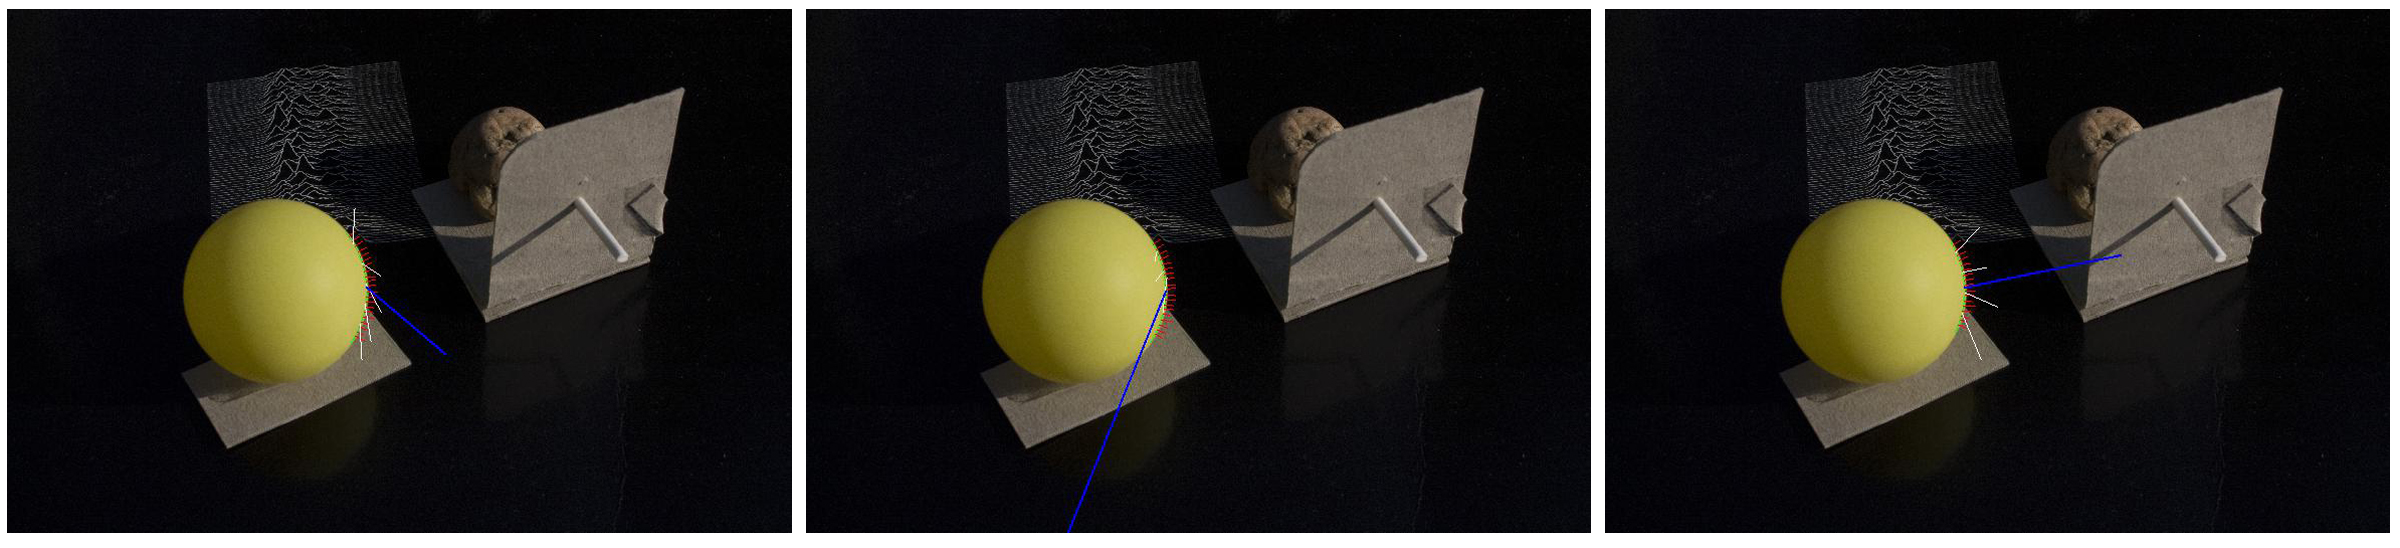
\includegraphics[width=\linewidth]{Images/Lage_der Subcontour.jpg}
	\caption[Bildunterschrift]{Results of slightly different sub-contours.}	
		\label{fig:subcontourRes}	
\end{figure}

The more complex objects of the second batch are evaluate as well and displayed in Figure~\ref{fig:complexRes}. Here, the image show obviously the randomness of the estimated vectors as well. Especially at the points where the contour changes significantly the direction, the $\vec{L}^n$ seems to have extremely wrong estimations but those outliers can be recognised in the other images like the left one in Figure~\ref{fig:subcontourRes} or the middle one in Figure~\ref{fig:difDistance} as well. Hence, the shape of the sub-contour seems to have no influence to the quality and robustness of the Johnston approach.
\begin{figure}[H] 
	
	\center 
	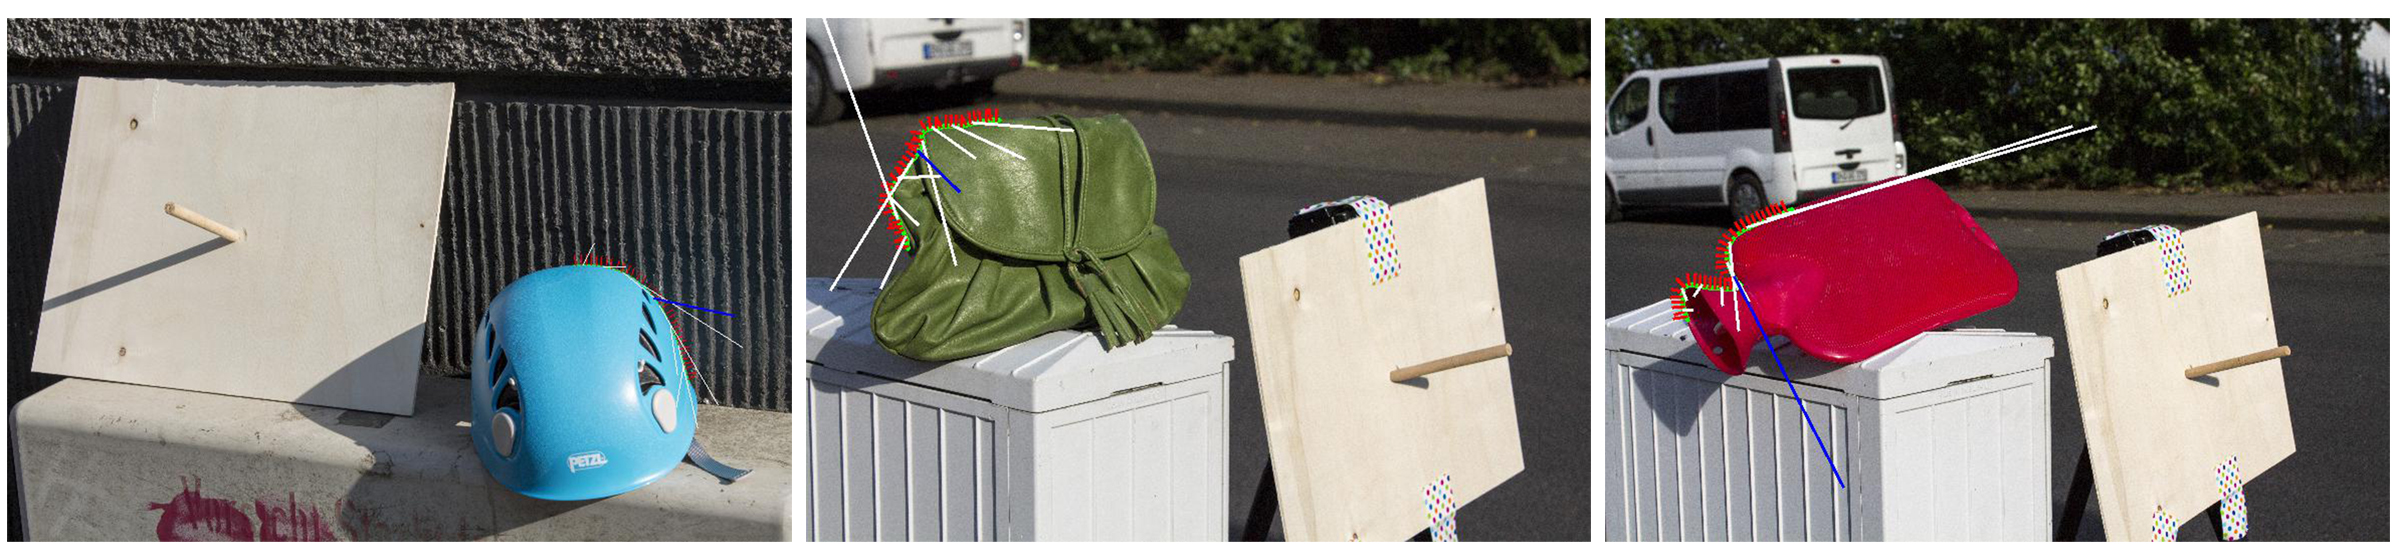
\includegraphics[width=\linewidth]{Images/Komplex_res.jpg}
	\caption[Bildunterschrift]{Results of more complex objects.}	
	\label{fig:complexRes}	
\end{figure}



\subsection{Evaluation 3. Approach}
Figure~\ref{fig:highRes} displays the results with the third approach which sets the light vector estimation $\vec{v}$ as  $\vec{L}^{max}$ of the patch with the maximum intensity. The directions seem to be as random as in the second approach and the algorithm lacks of robustness and continuity. Even the $\vec{L}^n$ of the images of the first batch point in various direction with no coherence and the significant outliers at contour points where the direction changes can be recognised. In case of the lower left image an almost correct light vector could be approximated as well. Another advantage is the more reproducibility of the final light vector when the sub-contour only differs slightly. These observations yields to the conclusion that there are no significant differences in quality and trustworthiness between both approaches. 
\begin{figure}[H] 
	\center 
	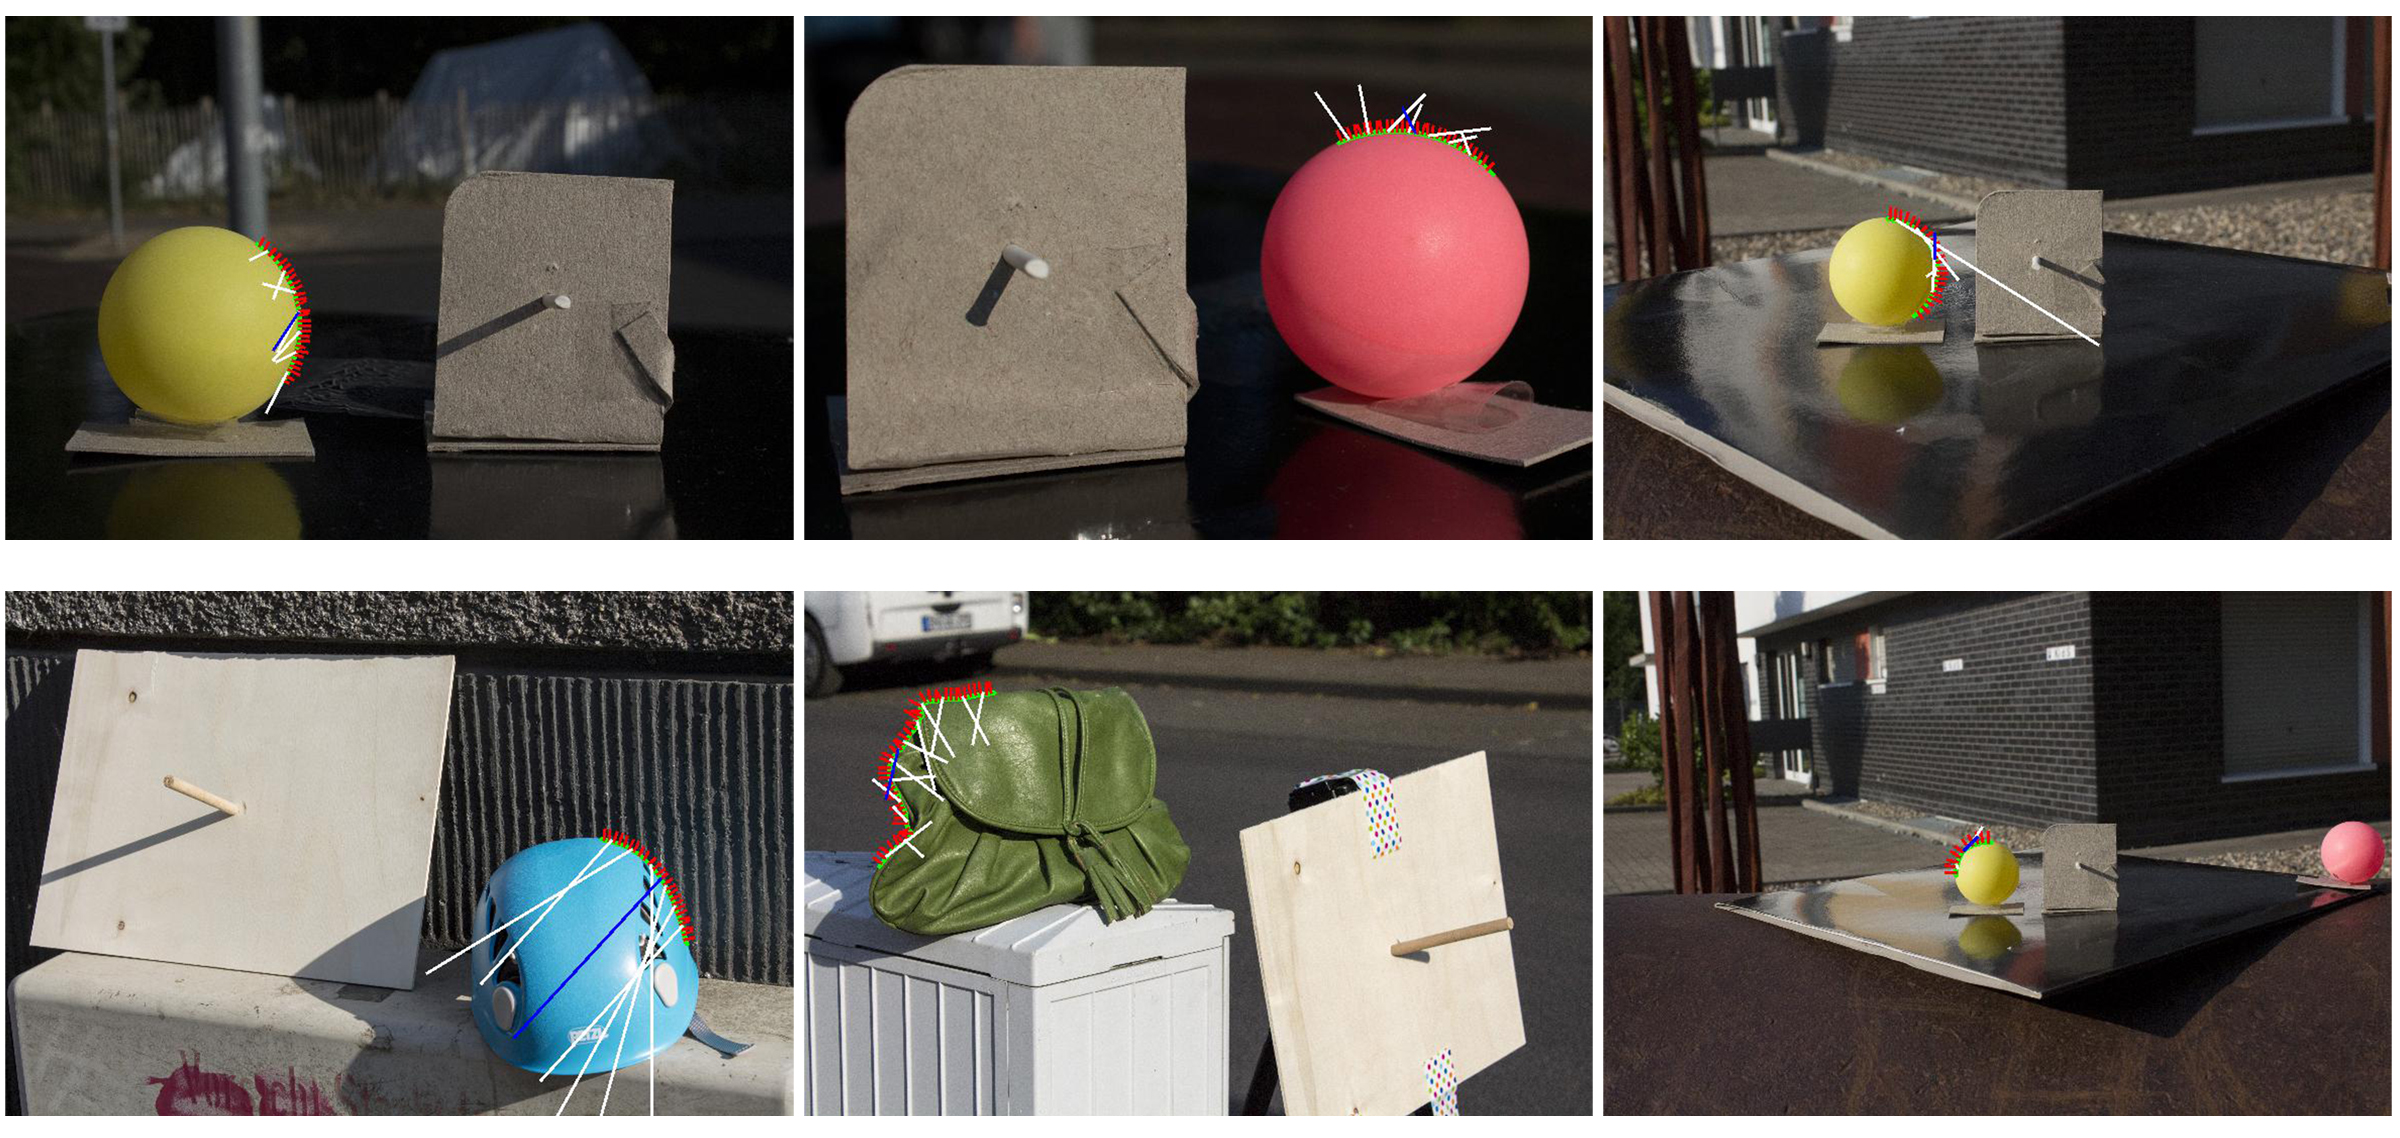
\includegraphics[width=\linewidth]{Images/High_res.jpg}
	\caption[Bildunterschrift]{Results of third approach with the light vector of the patch of highest intensity.}	
	\label{fig:highRes}	
\end{figure}


\subsection{Discussion of Evaluation Results}

The promised robust and correct results of Johnson~\cite{Johnson} can not be reproduced. It is obvious that the authors used very simple and homogeneous objects as well and did not display the patch related light vectors in the complex scenes like the image of prominent people. This leads to the suspicion that only the best results were publicized which could be occasionally estimated with the reproduced implementation, too. 

It has to be mentioned, that this evaluation is based on visual impressions, but the results differ very significantly from the validated sun clock light direction, and can be easily recognised. There were no evidences of correlations in the considered images and the final light vectors seems to point into none comprehensible directions. This randomness is proofed by the sensibility of slightly different sub-contours which influence the results vastly. Other assumptions like the influence of the image section size or problems with special angles between $\vec{N}$ and $\vec{L}$ can not be confirmed, beside the horizontally flipped vectors if the angle is in the range of  $0^\circ $ and $-90^\circ$. 

The comparison of the second and third approach proofs enhance the assumption that the lack of robustness is related to external influences. Those can be additional reflections at surfaces in the direct neighbourhood of the object of interest or a specular highlight in the proximity of the outer object boundary that forge the constant reflection assumption. These assumptions were made in Section~\ref{sec:lightingmodel} to simplify the approximation problem in Equation~\ref{equ:Blinn}. It discards completely the existence of specular reflection parts and the fact that surfaces reflects not ideal isotropic in reality. Another failure is the ignition of surface reflections in the object's environment that can be interpreted as additional light sources which forge the pixel intensities as well. 

In addition, it can not be figured out if the complexness of the object's shape has any influence of the quality, because of the lacking correlation. The recognised outliers can be observed in the results with the perfect round and even contours of the second bath\textcolor{red}{=batch??} as well. Therefore, it is challenging to get a conclusion about the influence of patches at direction changing contour points because they can be extremely outliers and no regularity.

A totally different hint to the none usefulness of this two dimensional approach can be the lack of publications from other authors that work with this method. Most of all other published methods work with multiple views and solve three dimensional problems to estimate the light direction. Thus, it can be assumed that maybe the conversion in a two dimensional space leads to the high lost of precision.

\subsection{Conclusion of Evaluation}
Hence, it can be considered that the previously made assumptions to simplify the approximation problem do not stand in reality. This model is related to perfect laboratory conditions and objects with an even surface that reflects nearly isotropically. It is obvious the reflections and other external influences distort the results in reality and thus the measuring of the intensity values along the sub-contour is not sufficient. No correlations could be made between the fault direction estimations that consider the lost of important information during the conversion into the two dimensional space. Therefore, it can be assumed that the results are not reliable and completely random.

Thus, the approach of Johnson~\cite{Johnson} is definitely not useful for professional validated image forgery. The promised results are not reproducible and this fact leads to the suspicion that only the best results were publicized.

\newpage